\chapter{Development Guide}

\section{Workflow}

\begin{figure}[h] 
	\centering
	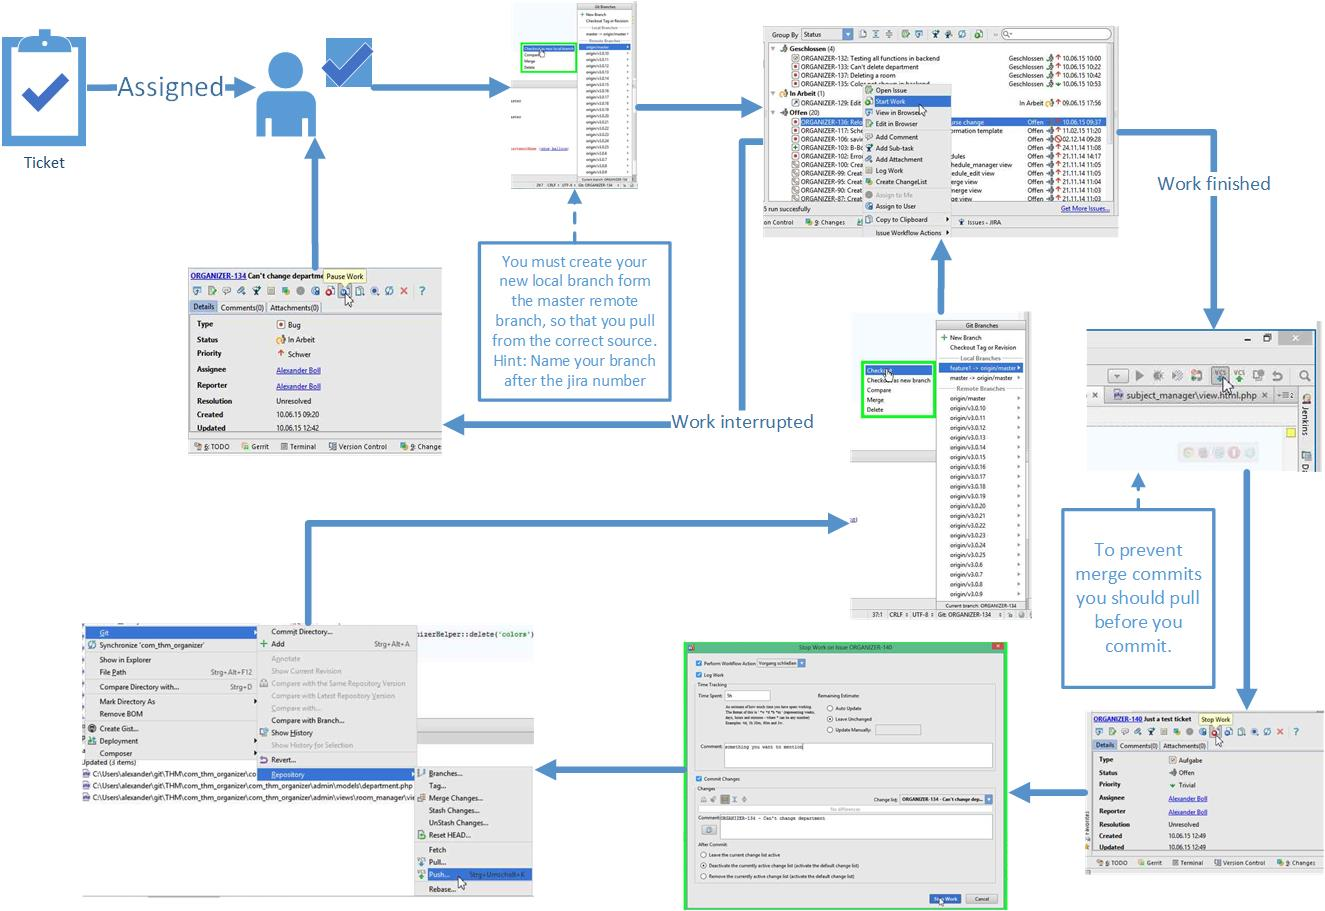
\includegraphics[width=14cm]{workflow.jpg}
	\caption{Gerrit Workflow}
	\label{fig:gerrit-workflow}
\end{figure}

\section{Developing}

\subsection{Advanced PHP Tips}
\subsubsection{String Equals Zero In PHP}
\footnote{Original text from: \url{http://www.hashbangcode.com/blog/string-equals-zero-php}}Due to the weakly-typed nature of PHP you can do some odd things, some of which are good, and some of which will enable you to shoot yourself in the foot. Care if you compare string with integer values. Take the following little snippet.

%\fvset{frame=single}
%\begin{pyglist}[language=php,numbers=left,numbersep=5pt]
%<?php
%$index = 0;
%var_dump($index == 'attributes'); //>bool(true)
%\end{pyglist}
%\fvset{frame=none}

Maybe you expect that the in-built function var\_dump() outputs bool(false) because 0 is not equal 'attributes' but instead the result is bool(true)! When you compare an integer and string, PHP converts the string to an integer. The integer of the string 'attributes' is 0. So var\_dump(0 == 0) outputs bool(true).

\section{Integration}

\subsection{Reviewing}

As a reviewer one has the responsibility of ensuring code quality. The Gerrit plugin offers many features which make this process easier. To open the Gerrit plugin's interface click on the icon on the bottom edge of the PHPStorm interface, as in \figref{fig:gerrit-plugin-interface}.

\newpage

\begin{figure}[h] 
	\centering
	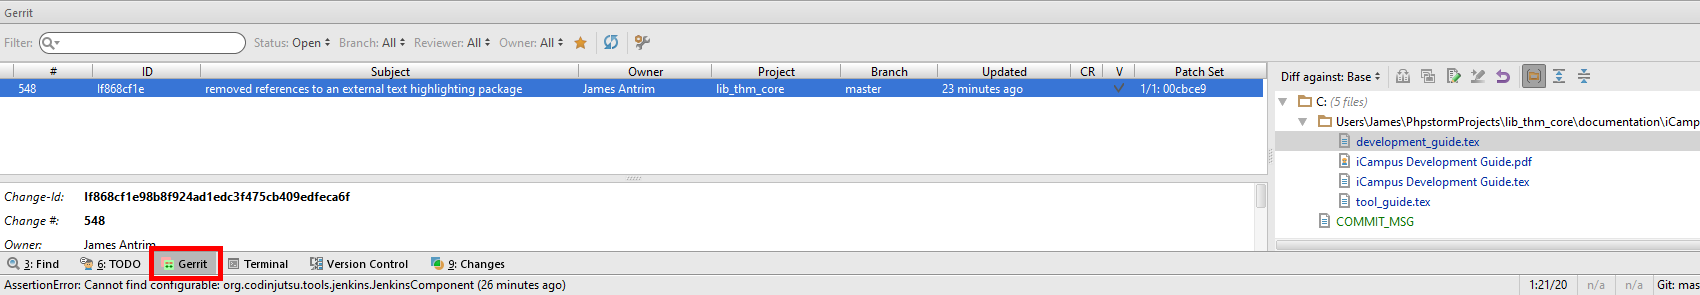
\includegraphics[width=14cm]{gerrit-plugin-interface.png}
	\caption{Gerrit Plugin Interface}
	\label{fig:gerrit-plugin-interface}
\end{figure}

\noindent
In this figure we see a previous commit already highlighted. This commit has already been examined by Jenkins and has been deemed to be of acceptable quality, this is evinced by the checkmark in the 'v' column. Jenkins can only performs automated tests and checks, which are good for problems which can be detected in this manner. It cannot find every error, and it is this point which the review system seeks to iron out, letting reviewers examine code before it is permanently made of a release.\\
\\
Because it is highlighted, the files changed by this commit are listed on the right hand side. To see the changes to individual files right click on the file in this list and select \texttt{Show Diff}.\\

\begin{figure}[h] 
	\centering
	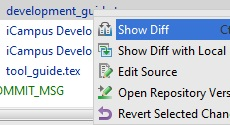
\includegraphics[width=6cm]{gerrit-plugin-file-review.png}
	\caption{File Review Interface}
	\label{fig:gerrit-plugin-file-review}
\end{figure}

\noindent
This opens a further interface where the local contents are then compared with those in the change. A review can then examine changes line by line to ensure the desired code quality has been reached. At this point multiple options open, but only the most important will be described.\\

\subsubsection{Approval}

Should the code be of an acceptable quality the reviewer can merge the commit with the master branch by right clicking on the list entry, opening the context menu (\figref{fig:gerrit-plugin-context-menu}). Then the reviewer can 'review' the commit by hovering over the word \texttt{Review} to the right a sub menu opens in which he selects \texttt{$+2$}. This tells Gerrit that the code has been reviewed and approved. By right-clicking again on the entry and left-clicking on submit the commit will then be merged into the master branch.

\begin{figure}[h] 
	\centering
	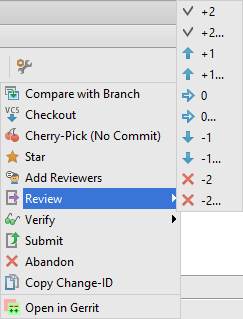
\includegraphics[width=5cm]{gerrit-plugin-context-menu.png}
	\caption{Commit Context Interface}
	\label{fig:gerrit-plugin-context-menu}
\end{figure}

\subsubsection{Rejection}

If the code needs improvement it can either be rejected outright or fixed. Outright rejection is performed over the same context menu as approval, only instead of \texttt{$+2$}, the reviewer then selects \texttt{$-2$} or \texttt{$-2$...}. The second option allows for a rejection message, which can be useful for stating the reason why the commit was rejected.\\
\\
The other option is to correct or improve the commit. To do so, the reviewer opens the commit context menu and selects \texttt{Checkout}. This creates a new local branch with the same stand as the commit to be corrected or improved. In the bottom right hand corner of the PhpStorm interface the new branch is now displayed. Click on the branch name to open the branch-interface. Select master and in the context menu that opens select \texttt{Checkout}. This sets your repository to the stand of the current master branch. Next reopen the branch-interface and click on the newly created local branch. In the menu that now opens select \texttt{Merge}. This merges that changes from the new branch onto the stand of the master.\\
\\
Now that you have the commit's changes in your master branch proceed to correct and improve the changed files as appropriate. When you have completed your changes append them to the previous commit by placing the checkmark in the \texttt{Append Commit} box and performing the commit and push as you normally would.

\newpage
\section{Testing}
\footnote{Source: Rost, Wolf (2014): Software Tests in Agile Web-CMS Development. TH-Mittelhessen.}The black box in Figure \ref{test_folder_structure} shows the repository structure with the extension and test folder structure. The tests are separated by unit and GUI tests. Integration tests are also stored in the unit-tests folder. Should it be necessary, they could also be in a separate folder. The green box in Figure \ref{test_folder_structure}  shows the unit-tests folder in more detail. This folder is structured into a general part (\textit{schema} and \textit{stubs}) and the two folders \textit{admin} and \textit{site}. The folder \textit{admin} contains the tests for the back-end of the extension. And also the test suite (phpunit.xml) and the bootstrap (component\_bootstrap.php) file. The \textit{site} folder is structured like the \textit{admin} but has the unit tests for the front-end of the extension in it. Both folders have to include a bootstrap file because some Joomla path constants are different for the back-end and the front-end. \newline
The folder \textit{schema} includes the database schema file (ddl.sql). The database schema is written in SQLite syntax\footnote{See \url{http://www.sqlite.org/lang.html}, stand 31.08.2014}. This file is used by the tests to create the SQLite database tables. \newline
Directly under the \textit{stubs} folder files are located that contain data for the tests. For instance, a long text or a JSON string is stored, to keep the tests readable. The folder \textit{database} contains files in which the database entries are stored. The entries are loaded by the tests and stored into the SQLite database tables. \newline
The blue box in Figure \ref{test_folder_structure} shows the gui-tests folder in more detail. Like the unit-tests folder, the gui-tests folder is divided into a back-end (admin) and a front-end (site) part. The \textit{Pages} folder contains classes that implements the Page Object pattern. The bootstrap file (component\_bootstrap.php) is the same for the back-end and front-end. This file registers the classes in the \textit{Pages} folder so that the GUI tests can use them without explicitly include them.

To be able to execute the tests, they must be copied to the \textit{tests} folder in an Joomla instance. Figure \ref{test_folder_structure_joomla} shows the file structure of the \textit{tests} folder in an Joomla instance. This folder also includes the basic TestCase classes (tests/core/case), Hard-Coded Mock Objects (tests/core/mock) for general Joomla objects (JApplication, JConfig, JDocument, JLanguage, etc.) and a reflection helper class (tests/core/reflection) to get private and protected values in a class by reflection\footnote{See \url{http://php.net/manual/de/book.reflection.php}, stand 31.08.2014}. \\ 
In addition, the folder contains Page Objects classes (tests/Pages) for all GUI tests because they represent webpages, which all extensions can use, like the login page, the control panel in the back-end and more. Furthermore there are iCampus Page Objects classes (test/Pages/icampus) that provide methods for general tasks, like add/edit/delete an item in a manager view in the back-end. The last folder (tests/SeleniumClient) contains the PHP-SeleniumClient which allows to interact with the Selenium server. The file bootstrapJ3.php includes the Joomla framework and registers the TestCase classes. This file is again included by the component\_bootstrap.php file (tests/com\_thm\_organizer/unit-tests/admin \& site). The bootstrapSelenium.php file makes the general Page Object classes available for the GUI tests and includes the JoomlaWebdriverTestCase.php. This file is the superclass of the GUI test classes and initialises a WebDriver object (SeleniumClient) using the configuration in the seleniumConfig.php file. All the general folders in the tests folder except the com\_thm\_organizer folder are stored in the joomla\_ci repository (\footnote{joomla\_ci repository: \url{http://dev.mni.thm.de/gitblit/summary/ci!joomla_ci.git}}) in GITBlit. Jenkins and the developers just have to copy the general folders from the CI repository and the tests from the extensions repository to an instance of Joomla and can immediately execute the tests. The requirements to execute the tests are listed below. Almost always the requirements are met on the machines of developers. 
\begin{itemize}
\item PHPUnit 4.0 (minimum)\footnote{See \url{https://phpunit.de/manual/current/en/installation.html}, stand 19.01.2014}
\item PHP 5.4 (Joomla also requires PHP)\footnote{See \url{http://www.joomla.org/technical-requirements.html}, stand 01.09.2014}
\item An Joomla 3 instance with the installed extensions.
\item SQLite3 (Is enabled by default.)
\end{itemize}
	
\begin{figure}
\centering
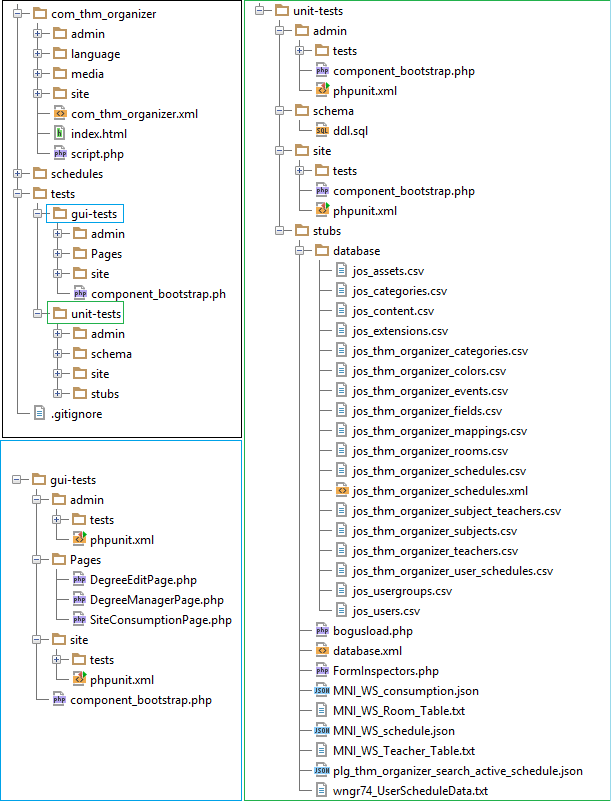
\includegraphics[scale=0.80]{images/test folder structure}
\caption[Caption for LOF]{Repository file structure of the THM Organizer component. The black box gives an overview of the file structure. The blue box shows the gui-tests folder in detail. The green box shows the unit-tests folder in detail.{\footnotesize (Source: Rost, Wolf (2014): Software Tests in Agile Web-CMS Development. TH-Mittelhessen.)}}

\label{test_folder_structure}
\end{figure}


\begin{figure}
\centering
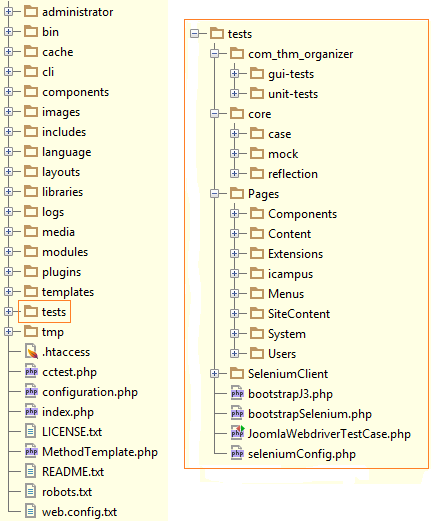
\includegraphics[scale=0.8]{images/test folder structure in joomla}
\caption[Caption for LOF]{Test folder structure of an Joomla instance.{\footnotesize (Source: Rost, Wolf (2014): Software Tests in Agile Web-CMS Development. TH-Mittelhessen.)}}
\label{test_folder_structure_joomla}
\end{figure}